\section{Visual exploration of data}
\begin{frame}
    \frametitle{An introduction to PowerBI}
\begin{block}{A report generator}
    \begin{itemize}
        \item<+-> Power BI is a reporting and data analytics tool.
        that simplifies data collection, transformation, 
        and visualization tasks.
        \item<+-> It is designed to be extensible and tends has become
        the de facto standard in the industry.
    \end{itemize}
\end{block}
\begin{block}{What PowerBI is not}
    \begin{itemize}
        \item<+-> While it performs well in terms of data visualization,
         it is not a full-fledged statistical software.
        \item<+-> The use of a superior data transformation
         and analysis tool is a highly effective strategy.
    \end{itemize}
\end{block}    i
\end{frame}
\begin{frame}
    \frametitle{R}
\begin{block}{The workhorse of statistics}
    \begin{itemize}
        \item<+-> A free and open source piece of software.
        \item<+->R boasts implementation of nearly all developments in statistics.
        \item<+-> The number of free programs written in R is keeping increasing.
    \end{itemize}
\end{block}
\begin{block}{A companion to PowerBI}
    \begin{itemize}
        \item<+-> PowerBI can collect data from a R script.
        \item<+-> PowerBI can transform data using a R script.
        \item<+-> PowerBI can display the output of a R script. 
    \end{itemize}
\end{block}    
\end{frame}
\begin{frame}
    \frametitle{R in a nutshell}
\begin{block}{R as a desk calculator}
    \begin{itemize}
        \item<+-> Open R by double-clicking on the R icon.
        \item<+-> Simply type "2+3" and observe the result.
        \begin{figure}[htbp]
            \centering
            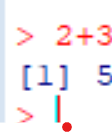
\includegraphics[scale=0.5]{R-sum.png}
            \caption{A simple sum}
            \label{<label>}
        \end{figure}
        \item<+-> A value  can be stored in
        a variable with the operator \texttt{<-}.
        \begin{figure}[htbp]
            \centering
            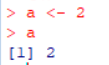
\includegraphics[scale=0.5]{variable.PNG}
            \caption{Using a variable.}
            \label{fig:variable}
        \end{figure}
    \end{itemize}
\end{block}
\end{frame}
\begin{frame}
    \frametitle{Vectors}
\begin{block}{Vectors}
    \begin{itemize}
        \item<+-> Vectors are created using the "c" (concatenate) or range operator "min:max".
        \item<+-> Try "c(0.1, 2, 3)" and "1:100".
        \item<+-> If you want a non-unit step, use the "seq(min, max, step)" command.
        \begin{figure}[htbp]
            \centering
            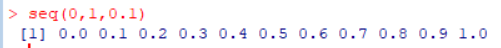
\includegraphics[scale=0.5]{seq_example.png}
            \caption{User-defined step}
            \label{fig:arbitrary_range}
        \end{figure}
        \item<+-> All the elements of a vector must be of the same type:
        numeric (double, integer, complex), logical, string.
    \end{itemize}
\end{block}
\end{frame}
\begin{frame}
    \frametitle{Vectors}
    \begin{block}{Numeric and boolean types}
        \begin{itemize}
            \item<+-> By default, a numeric value is encoded 
            as a double precision number on 64 bits. 
            \item<+-> A complex number is declared with syntax $x + yi$:
           \begin{figure}[htbp]
            \centering
            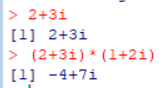
\includegraphics[scale=0.5]{complex_number.PNG}
            \caption{Complex numbers}
            \label{fig:complex_numbers}
           \end{figure}
           \item<+-> Booleans are TRUE or FALSE.
           \begin{figure}[htbp]
            \centering
            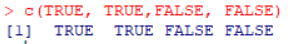
\includegraphics[scale=0.5]{boolean.PNG}
            \caption{Booleans}
            \label{fig:booleans}
           \end{figure}
        \end{itemize}
    \end{block}
\end{frame}
\begin{frame}
    \frametitle{Vectors}
    \begin{block}{Character strings}
        \begin{itemize}
           \item<+-> A string is enclosed with double or simple quotes.
           \begin{figure}[htbp]
            \centering
           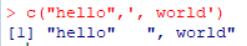
\includegraphics[scale=0.5]{string.PNG} 
            \caption{Character strings}
            \label{fig:char_strings}
           \end{figure}
           \item<+-> Any R object can be converted to an informative string with the function
           \texttt{str().}
        \begin{figure}[htbp]
            \centering
           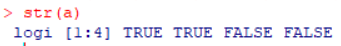
\includegraphics[scale=0.5]{str_func.PNG} 
            \caption{Str function.}
            \label{fig:str_func}
           \end{figure}
        \end{itemize}
    \end{block}
\end{frame}

\begin{frame}
    \frametitle{Vectors}
\begin{block}{Operators}
   \begin{itemize}
    \item<+->Operators and functions are applied elementwise.
     \begin{figure}[htbp]
            \centering
           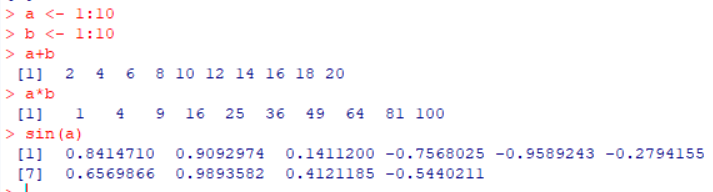
\includegraphics[scale=0.5]{vector_functions.PNG} 
            \caption{Operating on vectors.}
            \label{fig:vect_op}
           \end{figure}
    \item<+-> This is true also for comparison operators.
     \begin{figure}[htbp]
            \centering
           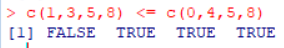
\includegraphics[scale=0.5]{comparison.PNG}
            \caption{Comparison operators.}
            \label{fig:vect_comp}
           \end{figure}
   \end{itemize} 
\end{block}
\end{frame}
\begin{frame}
    \frametitle{Vectors}
    \begin{block}{Accessing elements}
        \begin{itemize}
            \item<+-> An element in a vector can be referred to by its 
            index.
     \begin{figure}[htbp]
            \centering
           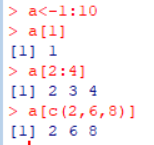
\includegraphics[scale=0.5]{elements.PNG}
            \caption{Accessing elements.}
            \label{fig:vect_elts}
           \end{figure}
           \item<+-> A selection by booleans is also possible.
           \begin{figure}[htbp]
            \centering
           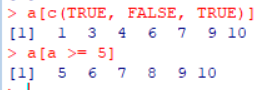
\includegraphics[scale=0.5]{bool_select.PNG}
            \caption{Boolean selection.}
            \label{fig:vect_bool}
           \end{figure}
        \end{itemize}
    \end{block}
\end{frame}
\begin{frame}
    \frametitle{Data frames}
\begin{block}{A convenient object.}
    \begin{itemize}
        \item<+-> Data frames are arrays holding observed values.
        \item<+-> Observed characteristics are in columns, observations in rows.
        \item<+-> The columns are named and can be referred to by their names.
        \begin{figure}[htbp]
            \centering
           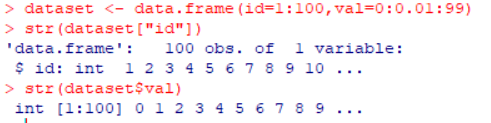
\includegraphics[scale=0.5]{dataframe.PNG}
            \caption{A data frame.}
            \label{fig:data_frame}
           \end{figure}
        \item<+-> Data frames are used by PowerBI to communicate with R.
    \end{itemize}
\end{block}
\end{frame}
\begin{frame}
    \frametitle{Passengers dataset}
    \begin{block}{Data collection}
        \begin{itemize}
            \item<+-> The dataset, collected from the site \url{https://data.europa.eu/data/datasets?locale=en}
            is stored in the file \texttt{avia\_paoc\_monthly.csv} that can be retrieved on ecampus in the folder \texttt{Datasets}.
            \item<+-> Launch PowerBI and select \texttt{Get data from other sources}.
            \item<+-> Select \texttt{Text/CSV} and open the file.
            \item<+-> A table view of the dataset appears.
        \end{itemize}
    \end{block}
\end{frame}
\begin{frame}
    \frametitle{Passengers dataset}
    \begin{block}{Data transformation}
        \begin{itemize}
            \item<+-> PowerBI offers the opportunity to transform the data.
            \begin{figure}[htbp]
                \centering
                
\includegraphics[scale=0.3]{power_bi_transform_data.png}
                \caption{Data transform.}
                \label{fig:data_transform}
            \end{figure}
            \item<+-> We are only interested in the total number of passengers carried by country, so all the rows
            below row 32 must be removed.
            \item<+-> Select \texttt{Keep rows}, then \texttt{Keep top rows} and finally enter 32. 
        \end{itemize}
    \end{block}
\end{frame}
\begin{frame}
    \frametitle{Passengers dataset}
    \begin{block}{Final transformations}
        \begin{itemize}
            \item<+-> In the first column, a description of the data includes at the end a geographic information. 
            \item<+-> Select the first column, right click on it, the select \texttt{replace values}.
            \item<+-> Copy all the text in the first cell, except the final two-characters country code.
            \item<+-> Keep the replacement text empty and click \texttt{replace}. 
        \end{itemize}
    \end{block}
   
    
\end{frame}
\begin{frame}
    \frametitle{Passengers dataset}
    \begin{block}{Transposing datasets}
        \begin{itemize}
            \item<+-> Datasets must have their values in columns.
            \item<+-> Select the tab \texttt{Transform}, then \texttt{Transpose}.
            \item<+-> Return to the \texttt{Home} tab and select \texttt{Use first row as headers}.
            \item<+-> The label of the first column is not very informative. Right click 
            on it and select \texttt{Rename}.
        \end{itemize}
    \end{block}

\end{frame}
\begin{frame}
    \frametitle{Passengers dataset}
\begin{block}{Cleaning data}
    \begin{itemize}
        \item<+-> A dataset may have blank row. Check yours and remove
        them if needed (\texttt{Remove rows} tab).
        \item<+-> Some values may be missing. In this dataset, they are coded 
        as ":". 
        \item<+-> The column "MK" has such values. Right click on it, then use 
        \texttt{Replace values} to change ":" by "0".
        \item<+-> finally, change the type of the column to \texttt{Whole number}.
    \end{itemize}
\end{block}    
   \begin{block}{Applying transforms}
    \begin{itemize}
        \item<+-> Select the \texttt{Close and apply} to apply the transforms.
        \item<+-> It is time to save your work (tab \texttt{File}) ! 
    \end{itemize}
   \end{block} 
\end{frame}
\begin{frame}
    \frametitle{Passengers dataset}
\begin{block}{Visual exploration of the dataset}
    \begin{itemize}
        \item<+-> Return to the \texttt{Home} tab, and start populating the report.
        \item<+-> Text boxes or visual can be added. 
        \item<+-> Select a text box and enter the text you wish to start your report.
        \item<+-> Select \texttt{New visual}. A new box appears (by default a bar chart).
        \item<+-> Select \texttt{Date} in the \texttt{Data} right pane and drag 
        the \texttt{Month} field to the visual. This defines the "x" axis.
        \item<+-> You can add data to your visual by selecting columns in the \texttt{Data} pane 
        or by dragging them. 
        \item<+-> Try changing the visual and see what happens.
    \end{itemize}
\end{block}
\end{frame}
\begin{frame}
    \frametitle{Passengers dataset}
\begin{block}{Data aggregation}
    \begin{itemize}
        \item<+-> In the "passengers" dataset, there is a one-to-one mapping
        between a month and the number of passengers. 
        \item<+-> What happens if we decide to plot against the quarter ?
        \item<+-> Uncheck \texttt{Month} in \texttt{Date} on the right pane and
        select \texttt{Quarter}.
        \item<+-> The visual now displays the total number of passengers for each quarter.
        \item<+-> In the \texttt{Y axis} part of the \texttt{visualization} pane,
        try to change \texttt{Sum} to \texttt{Average}.
        \item<+-> The aggregation of values is an important feature in PowerBI.
    \end{itemize}
\end{block}
\end{frame}
\begin{frame}
    \frametitle{Passengers dataset}
\begin{block}{Measures}
    \begin{itemize}
        \item<+-> A measure is a value that can be computed from the dataset.
        \item<+-> It may be viewed as a practical implementation of a random variable,
        a concept introduced later in the course.
        \item<+-> Since measures are computed on-the-fly, they always reflect the most up-to-Date dataset.
        \item<+-> Using them is a must in PowerBI.
        \item<+-> Create a \texttt{New quick measure} on the "passengers" dataset that sums the amount of 
        carried passengers by quarter for a given country (select the one you prefer).
        \item<+-> Use a visual to plot the result.
        \item<+-> Custom measures can be used, provided you know the "DAX" language.
    \end{itemize}
\end{block}
\end{frame}
\begin{frame}[fragile]
    \frametitle{PowerBI and R}
\begin{block}{R as a data source}
    \begin{itemize}
        \item<+-> Open the \texttt{Get data} tab, then select \texttt{R}.
        \item<+-> In the script box, type:
        \begin{lstlisting}{language=R}
dataset <- data.frame(x=1:100,y=runif(n=100,min=0,max=10))
        \end{lstlisting}
        \item<+-> Observe the result in PowerBI. What happens if the name \texttt{dataset} for the ouput variable is changed ?
        \item<+-> Create two data frames in the R script: what happens in PowerBI?
    \end{itemize}
\end{block}
\end{frame}
\begin{frame}[fragile]
    \frametitle{PowerBI and R}
\begin{block}{R as a data processor}
    \begin{itemize}
        \item<+-> Open the \texttt{Get data} tab, then select \texttt{Run R script}.
        \item<+-> In the script box, type:
        \begin{lstlisting}{language=R}
output <- dataset
output$z <- as.numeric(dataset$y)+1
        \end{lstlisting}
        \item<+-> A new column named \texttt{z} was added and its values are those of column \texttt{y} plus 1.
    \end{itemize}
\end{block}
\end{frame}
\begin{frame}[fragile]
    \frametitle{PowerBI and R}
\begin{block}{Visuals}
    \begin{itemize}
        \item<+-> On the \texttt{visualizations} pane, select the \texttt{R} icon.
        \item<+-> Drag the \textt{y} field in the visual.
        \item<+-> In the script box, type:
        \begin{lstlisting}{language=R}
hist(dataset$y)
        \end{lstlisting}
        \item<+-> An histogram is displayed in the visual. 
        \item<+-> This may be useful when a given visual, like the histogram, is not implemented in PowerBI or requires a plugin.
    \end{itemize}
\end{block}
\end{frame}
    
